\documentclass[danish]{article}
\usepackage[utf8]{inputenc}
\usepackage[danish]{babel}
\usepackage[T1]{fontenc}	

\usepackage[version=3]{mhchem} % Package for chemical equation typesetting
\usepackage{siunitx} % Provides the \SI{}{} and \si{} command for typesetting SI units
\usepackage{graphicx} % Required for the inclusion of images
\usepackage{subcaption} % Add the possibility for subfigures/subcaptions.
\usepackage{natbib} % Required to change bibliography style to APA
\usepackage{amsmath} % Required for some math elements

\usepackage{float}
\graphicspath{ {graphics/} }

\setlength\parindent{0pt} % Removes all indentation from paragraphs

\renewcommand{\labelenumi}{\alph{enumi}.} % Make numbering in the enumerate environment by letter rather than number (e.g. section 6)
\begin{document}

\title{\textbf{ Analog System Design }   Eksamensforberedelse}
\author{Jonas Lind}
\date{03-06-2017}
\maketitle
\section{Effektforstærkerøvelse: DC}
\begin{itemize}
	\item Klasse AB 30W forstærker til \SI{8}{\ohm} højtaler.
	\item Indgangsignalet har signalamplitude på 1V.
\end{itemize}

\paragraph{Spændingsvinget} som er nødvendigt for at drive højtaleren ved 30W beregnes til 22V. Der skal være plads til to basis-emitter strækninger for udgangstrinnet, noget lignende til den øvrige elektronik og ripple i effektforsyningen og  \SI{10}{percent}  på netspændingen så effektforsyningen bør placeres cirka 5V højere end kravet til $V_O$ og det giver værdien til $+-27V$.

\begin{equation}
P_O = \dfrac{U_{RMS}}{R_L}
\end{equation}

\begin{equation}
U_{RMS} = \sqrt{P_O R_L} = \sqrt{\SI{30}{\watt} \SI{8}{\ohm}} = \SI{15.5}{\volt}
\end{equation}

\begin{equation}
U_{PEAK} = U_{RMS} \sqrt{2} = \SI{22}{\volt}
\end{equation}
\paragraph{Strømsvinget} som er nødvendigt på forstærkerens udgang igennem de \SI{8}{\ohm} findes til at være \SI{3.65}{\ampere}, ved en nominel modstandsværdi på \SI{6}{\ohm}. Dette er gældende da højttalerens svingspole har en DC modstand $R_{DC}$ på typisk \SI{80}{percent}  af den nominelle værdi.

\begin{equation}
I_{O\,PEAK} = \dfrac{U_{PEAK}}{R_L} = \SI{3.65}{\ampere}
\end{equation}

\paragraph{Udgangstrinnet} benytter et darlington par af to emitter følgere (common collector) for at øge strømforstærkningen. 

\begin{equation}
\beta = \beta_1 \beta_2 = 100 {\cdot} 30 = 3000
\end{equation}

\begin{itemize}
	\item Dette sænker de \SI{3.65}{\ampere} udganstrinnet skal levere til \SI{1.22}{\milli\ampere}.
	\item Således belaster udgangstrinnet VAS-trinnet minimalt.
	\item En \SI{2}{\kilo\ohm} base-modstand begrænser basestrømmen til højest \SI{1.45}{\milli\ampere}.
	\item Modstanden er bestemt ved at se på fuldt udsving hvor højtaleren har \SI{22}{\volt} over sig og der er 3 gange \SI{0.7}{\volt} op til basen.
\end{itemize}

\begin{equation}
R = \dfrac{\SI{27}{\volt} − (3 \cdot \SI{0.7}{\volt} + \SI{22}{\volt})}{\SI{1.22}{\milli\ampere}} = \SI{2.38}{\kilo\ohm}
\end{equation}

\paragraph{Diode biasing} benyttes for at minimere crossover distortion. Fire dioder sættes i serie for at skabe et fast spændingsfald på \SI{2.8}{\volt} mellem de to transistores baser. 

\begin{figure} [H]
	\centering
	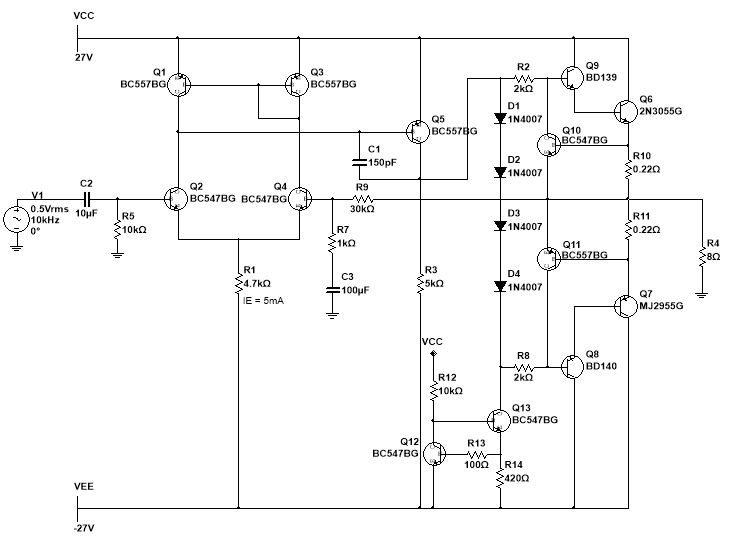
\includegraphics[width=\linewidth]{graphics/PowerAmp_schematic}
	\caption{Kredsløbsdiagram for effektforstærker klasse AB.}
	\label{fig:PowerAmp_schematic}
\end{figure}

\paragraph{Strømkilde}
For at levere strømmen til dioderne anvendes en strømkilde istedet for en modstand, da der vil blive afsat for meget effekt i denne.
Modstanden $R_E (R_{14})$ styrer $I_O$.
$R_{12}$ sørger for at der løber en strøm i dioderne, der giver et konstant spændingsfald.

\newpage
\section{Effektforstærkerøvelse: AC}

\subsection{Forstærkning og stabilitet}
\begin{itemize}
	\item Der laves en dominerende pol for at sikre stabilitet ved at forstærkningen er sænket til under 1 når fasedrejet er 180°.
	\item Dette begrænser forstærkerens båndbredde.
	\item Slew rate begrænsning af kondensatoren $C_C$ og strømmen $I_E$.
	\item Ved hurtig og stor udstyring bliver sinusen til en trekant pga den begrænsede hastighed.
\end{itemize}

\paragraph{Det strømforstærkende trin} benytter en BJT transistors strømforstærkning β for at forstærke differentialtrinnets udgangsstrøm. Denne strøm bliver ledet gennem en modstand, $R_C$, som laver det om til en strøm. 

I en integreret forstærker benyttes ofte flere transistorer til at forøge den resulterende strømforstærkning mens en effektforstærker som oftest nøjes med en enkelt transistor da der ikke er behov for den ekstremt høje forstærkning ved DC. 

\begin{figure} [H]
	\centering
	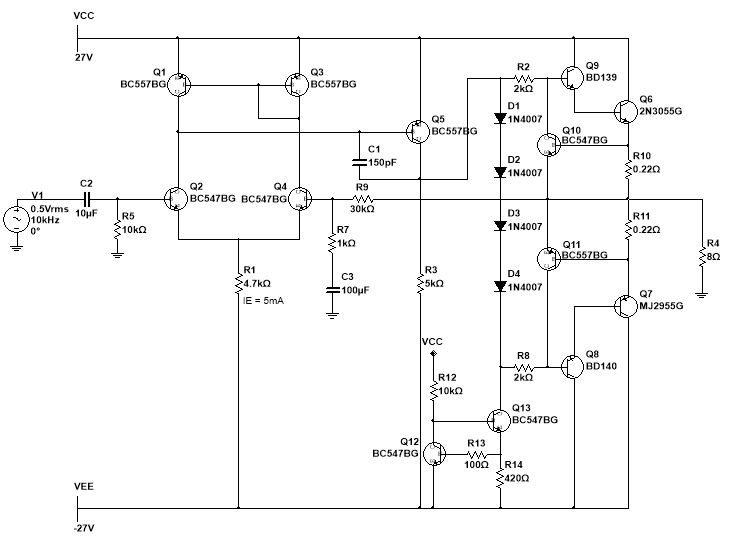
\includegraphics[width=\linewidth]{graphics/PowerAmp_schematic}
	\caption{Kredsløbsdiagram for effektforstærker klasse AB.}
	\label{fig:PowerAmp_schematic1}
\end{figure}
DC forstærkningen er således givet ved:
\begin{equation} 
A_{DC} = g_m \beta R_C
\end{equation}

Transkonduktansen gm i differentialtrinnet T1 ... T4 beregnes til 0,1 

Kondensatoren $C_C$ skaber en dominerende pol ved $f_0$, som sikrer stabilitet.

\begin{equation} 
f_0 = \dfrac{1}{2 \pi \beta R_C C_C}
\end{equation}

Slew-raten (SR) begrænses af kondensatoren og strømmen $I_E$.

\begin{equation} 
SR = \dfrac{I_E}{C_C}
\end{equation}

\begin{figure} [H]
	\centering
	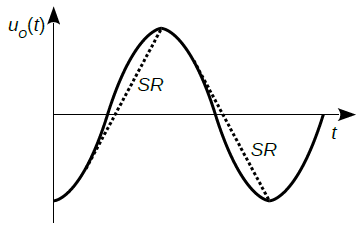
\includegraphics[width=0.65\linewidth]{graphics/slewrate}
	\caption{Operationsforstærkerens slew rate.}
	\label{fig:slewrate}
\end{figure}

Den dominerende pol giver stabilitet, men begrænser også hvor hurtigt udgangen kan flyttes. Hvis værdien forsøges overskredet bliver signalet forvrænget.

\subsection{Transistor - AC model}
\subsection{Diode - AC model}

\newpage
\section{Effektforstærkerøvelse: Effektafsættelse}
Herunder regnes den totale effekt afsat i forstærkeren og ud fra den findes effekten afsat i udgangstrinnet.\\

Den tilførte effekt på \SI{67}{\watt} ved \SI{30}{\watt} afgivet i nominelt \SI{8}{\ohm}. 

\begin{equation}
I_{O\,PEAK} = \SI{3.65}{\ampere}
\end{equation}

\begin{equation}
I_{DC} = \dfrac{I_{O\,PEAK}}{\pi} =\SI{1.16}{\ampere}
\end{equation}

\begin{equation}
P_{CC} = U_{CC}(I_{PEAK}-I_{DC})=\SI{67.2}{\watt}
\end{equation}

Effekttabet i udgangstransistorerne T9 og T10 bliver \SI{32}{\watt} samlet og derfor forventes et tab på \SI{16}{\watt} i hver transistor. 

\begin{equation}
P_O = \dfrac{U_{CC}U_O}{\pi R_L} =\SI{31.2}{\watt}
\end{equation}

\subsection{Ohms lov analogi}
En køleprofil beskrives normalt ved en termisk modstand og Ohms lov antages at gælde for det termiske system. 
Man siger at effektstrømmen $P$ løber gennem den termiske modstand $R_{th}$ og det danner et temperaturfald på $R_{th}P$ som hæver temperaturen $T$ over omgivelsestemperaturen $T_{amb}$.
Den termiske modstand kaldes undertiden for køleprofilets K-værdi og enheden er en stigning i temperatur per effekt.

\begin{figure} [H]
	\centering
	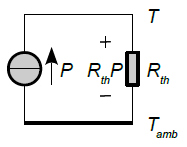
\includegraphics[width=0.65\linewidth]{graphics/ohmslovanalogi}
	\caption{Beregning af temperaturstigning ved en effektstrøm P i en termisk modstand.}
	\label{fig:ohmslovanalogi}
\end{figure}

\subsection{Termisk modstand}
\begin{itemize}
	\item Angiver evnen til at transportere og afsætte varme, f.eks. fra transistorens junction til dens overflade.
	\item Måles i \SIUnitSymbolCelsius /\si{\watt}
	\item Jo højere værdi, jo varmere vil et komponent blive ved en given afsat effekt.
\end{itemize}

Klasse AB forstærkerens effekttransistor junction ønskes kølet til maksimalt \SI{100}{\degreeCelsius}
Ifølge databladet for 2N3055 er junction to case = \SI{1.52}{\degreeCelsius\per\watt}.

\begin{equation}
T_j = (R_{th\:j-mb} + R_{th\: mb-hs} + R_{th\: hs})P + T_{amb}
\end{equation}

\begin{equation}
R_{th\: hs} = \dfrac{T_j-T_{amb}}{P}-R_{th\:j-mb} + R_{th\: mb-hs}
\end{equation}

\begin{equation}
R_{th\: hs} = \dfrac{\SI{100}{\degreeCelsius}-\SI{25}{\degreeCelsius}}{\SI{11}{\watt}}-\SI{1.52}{\degreeCelsius\per\watt} = \SI{5.3}{\degreeCelsius\per\watt}
\end{equation}

Til effekttransistorene blev der valgt en køleplade, som var rigeligt stor.

\subsection{SOA}
SOA er en betegnelse for safe-operating area.
SOA findes ved at kombinere følgende tre begrænsninger:
\begin{itemize}
	\item $I_{C,MAX}$
	\item  $U_{CE,MAX}$
	\item  $P_{MAX}$
\end{itemize}

$P_{MAX}$ giver skæringspunkterne for 2N3055:

\begin{equation}
I_C = \dfrac{P_{MAX}}{U_{CE}} = \dfrac{\SI{115}{\watt}}{\SI{60}{\volt}} = \SI{1.9}{\ampere}
\end{equation}

\begin{equation}
U_{CE} = \dfrac{P_{MAX}}{I_C} = \dfrac{\SI{115}{\watt}}{\SI{15}{\ampere}} = \SI{7.7}{\volt}
\end{equation}

\begin{figure} [H]
	\centering
	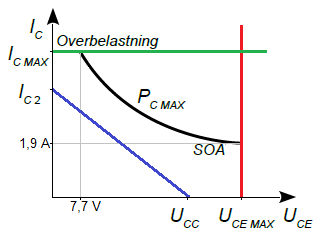
\includegraphics[width=0.65\linewidth]{graphics/soa}
	\caption{Safe-operating area.}
	\label{fig:soa}
\end{figure}

\newpage
\section{Effektforstærkerøvelse: Effektforsyning}

\subsection{Transformer}
\begin{itemize}
	\item En transformer kan regulere AC-spændinger (ikke DC!) op og ned.
	\item Lavere antal sekundær vindinger, giver en lavere udgangsspænding.
	\item Varmetab i spolerne \approx \SI{5}{percent}.
\end{itemize}


\subsection{Ensretning udglatning}
\begin{itemize}
	\item Full bridge brokoblingen ensretter de positive og negative halvbølger.
	\item Der er to diode-spændingsfald, som sænker spændingen \approx \SI{-1.4}{\volt}.
	\item Kondensatoren $C_{filter}$ udglatter den ensrettede spænding.
	\item Der vil være ripple, $U_{RIP}$, som øges ved større $I_O$.
	\item $U_{RIP}$ sænkes ved større kondensator.
	\item Elektrolyt-kodensator benyttes.
\end{itemize}

\begin{figure} [H]
	\centering
	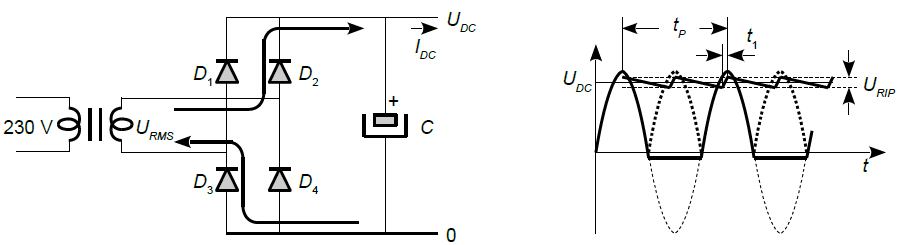
\includegraphics[width=\linewidth]{graphics/ensretter}
	\caption{AC fra transformeren ensrettet af brokoblingen.}
	\label{fig:ensretter}
\end{figure}


\begin{equation}
t_p = \dfrac{1}{\SI{50}{\hertz}} = \SI{20}{\milli\second}
\end{equation}

\begin{equation}
C_{Filter} = \dfrac{I_{DC}t_p}{2 U_{RIP}}
\end{equation}

\subsection{Serie regulator}
\begin{itemize}
	\item Lineær spændingsregulator, som afsætter overskydende spænding som varme.
	\item Input kondensatoren sikrer stabilitet, hvis dens forsyning er langt fra input.
	\item Output kodensatoren giver også stabilitet og evnen til hurtigt at levere strøm.
	\item Reguleres internt ud fra en bandgap spændingsreference, $V_{ref}$.
\end{itemize}

\begin{figure} [H]
	\centering
	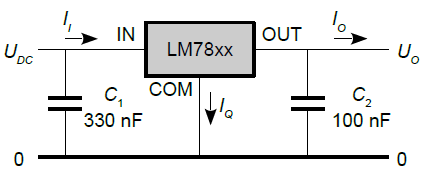
\includegraphics[width=0.8\linewidth]{graphics/serieregulator}
	\caption{En serieregulator der nedsætter spændingen fra en ustabil
		effektforsyning til en stabil og kortslutningssikker forsyningslinje. De viste kondensatorer er
		krævet af hensyn til stabilitet.}
	\label{fig:serieregulator}
\end{figure}

\subsection{DC-DC konverter}
DC konverteren benytter en spole til at optage energi fra indgangen i et kort tidsrum hvorefter energien overføres til udgangen i det efterfølgende tidsrum. 
Den proces gentages i en evindelighed styret af en transistor og en diode der arbejder som kontakter. 
Transistoren kan være bipolar eller felteffekt.
\begin{itemize}
	\item Kan regulere DC spændinger op og ned mere effektivt end lineære regulatorer.
	\item Har en virkningsgrad på over \SI{90}{percent}.
	\item Der er højfrekvent switching støj på udgangen, hvilket kan være uønsket.
\end{itemize}

\paragraph{Opkonvertering}
\begin{itemize}
	\item Et PWM signal med en frekvens > 100 kHz styrer MOSFET’en.
	\item Når MOSFET'en er tændt løber der en strøm igennem spolen, som oplades. C2 aflades. 
	\item Når MOSFET'en er slukket aflades spolen, som skaber en spænding i serie med $U_{DC}$, som lader C2 op igennem dioden.
	\item Dioden sørger for at kondensatoren ikke aflades tilbage igennem MOSFET’en.
	\item Gøres det hurtigt nok vil $U_O$ altid holdes over $U_{DC}.$
\end{itemize}

\begin{figure} [H]
	\centering
	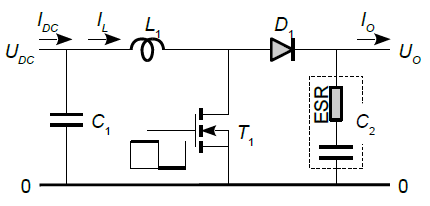
\includegraphics[width=0.8\linewidth]{graphics/opkonvertering}
	\caption{Opkonvetering.}
	\label{fig:opkonvertering}
\end{figure}

\paragraph{Nedkonvertering}
\begin{itemize}
	\item Ved nedkonvetering er der byttet rundt på MOSFET, diode og
	spole.
	\item Først når MOSFET’en er slukket løber der ingen strøm i kredsløbet.
	\item Når MOSFET’en tændes begynder strømmen langsomt at stige i spolen, det skaber et modsatrettet spændingsfald. Dette gør at $U_O < U_{DC}$.
	\item Imens strømmen stiger i spolen opbygger den et magnetisk felt.
	\item Når MOSFET’en slukkes vil spolen blive ved med at levere strøm, som opretholder udgangsspændingen.
\end{itemize}

\begin{figure} [H]
	\centering
	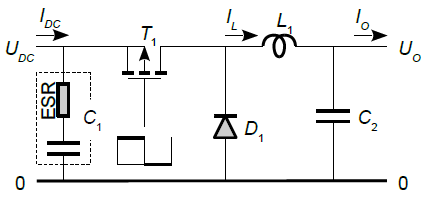
\includegraphics[width=0.8\linewidth]{graphics/nedkonvertering}
	\caption{Nedkonvetering.}
	\label{fig:nedkonvertering}
\end{figure}

\begin{equation}
C_{Filter} = \dfrac{I_{DC}t_p}{2 U_{RIP}}
\end{equation}


\newpage 
\section{Operationsforstærkeren}
En OpAmp kan beskrives ved et differentielt indgangstrin der omsætter en spænding til en strøm ved transkonduktansen $g_m$ og en strømforstærker $\beta$ der danner en spænding over $R_C$.

\begin{figure} [H]
	\centering
	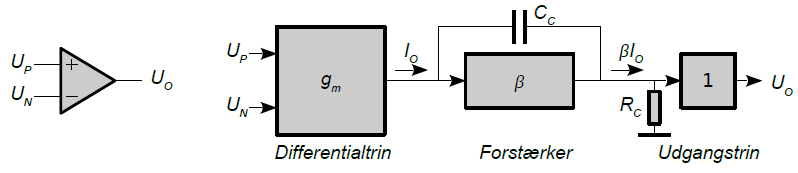
\includegraphics[width=\linewidth]{graphics/opamp_trin}
	\caption{En OpAmp består af et differentielt indgangstrin og en strømforstærker.}
	\label{fig:opamptrin}
\end{figure}

\begin{itemize}
	\item Forstærker forskellen mellems den to indgange, $U_P$ og $U_N$.
	\item Differential-trinnet laver spændingsforskellen om til en strøm $I_O$.
	\item VAS-trinnet forstærker strømmen med $\beta$, som laves til en spænding med $R_C$.
	\item Udgangstrinnet er en unity gain buffer, så udgangen af VAS-trinnet ikke belastes af eksternt load.
	\item Kondensatoren $C_C$ skaber en dominerende pol, der gør OpAmp’en stabil.
	\item DC gain: $A_{DC} = g_m \beta R_C$
	\item AC gain: $A_{OL} = \dfrac{g_m}{\omega C_C}$
\end{itemize}
\newpage 
\subsection{Opbygning og DC forhold}
\begin{itemize}
	\item Trin 1 – Spænding til strøm – en transkonduktans blok.
	\item Trin 2 – Forstærker strøm og omsætter til spænding - en transresistans forstærker, også kaldet VAS – Voltage Application Stage).
	\item Trin 3 – Kommer ved effektforstærkeren. Omsætter fra mA niveau til A niveau.
\end{itemize}

\begin{figure} [H]
	\centering
	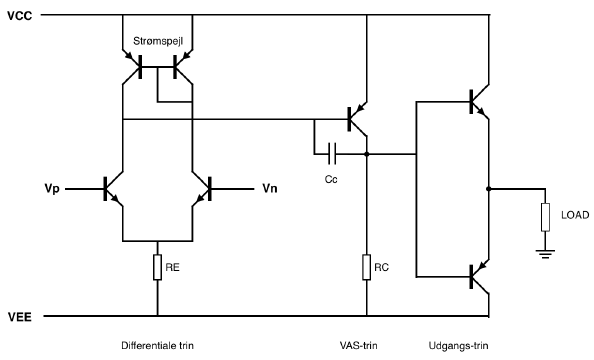
\includegraphics[width=\linewidth]{graphics/opamp}
	\caption{Generelt OpAmp kredsløb.}
	\label{fig:opamp}
\end{figure}
\newpage 
\paragraph{Differentialtrinnet} benytter to BJT med fælles emitter, en såkaldt differentielkobling. En strømkilde driver en fast strøm $I_E$ i den fælles emitter. De to transistorer tvinges derfor til at dele strømmen mellem sig. De to transistorer T3 og T4 udgør et strømspejl hvor strømmen i T1 kopieres over til T4. 

\begin{figure} [H]
	\centering
	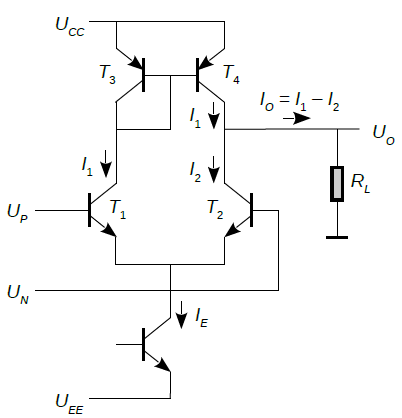
\includegraphics[width=0.68\linewidth]{graphics/differentialtrin}
	\caption{Differentialtrin med strømspejl.}
	\label{fig:differentialtrin}
\end{figure}
	
Strømdelingen styres af en spændingsdifferens $U_P – U_N$ mellem de to indgange ved basis. Hvis spændingsdifferensen er nul deles strømmen ligeligt med \SI{50}{\percent} til hver transistor. 
Hæves spændingsdifferensen vil T1 trække mere strøm og T2 må så nøjes med en mindre strøm da $I_E$ er konstant. 
På grund af strømspejlet ved T3 og T4 vil differensen mellem I1 og I2 give en strøm $I_O$ i udgangen.
	
Ved stor positiv spændingsdifferens vil T1 lede \SI{100}{percent} strømmen og T2 får \SI{0}{percent}. Der er derfor en øvre grænse for den strøm der kan løbe i udgangen. Det er ikke muligt at få en udgangsstrøm $I_O$ på mere end $I_E$ uanset spændingsdifferensen. 

\begin{equation} 
I_o = g_m(U_P-U_N)
\end{equation}

\begin{equation} 
U_T = \frac{k T}{q_0} \approx \SI{26}{\milli\volt}
\end{equation}

\begin{equation} 
g_m = \frac{I_E}{2nU_T}
\end{equation}
	
\begin{figure} [H]
	\centering
	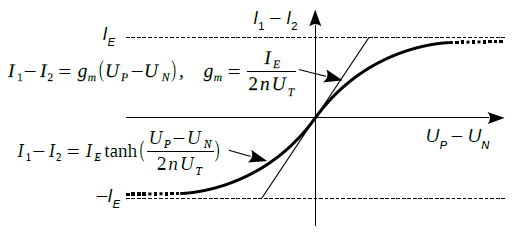
\includegraphics[width=0.8\linewidth]{graphics/differentialtrin_transkonduktans}
	\caption{Differentialtrinnets emitterstrøm.}
	\label{fig:differentialtrin_transkonduktans}
\end{figure}

Der er et næsten retlinet forløb for en spændingsdifferens nær ved nul og at stor spændingsdifferens giver et mætningsforløb for strømdifferensen I1 – I2 hvor der optræder en begrænsning til den fælles strøm i emitter. 

$I_E$ er arbejdsstrømmen, en emitterstrøm. Typisk \SI{100}{\micro\ampere} i operationsforstærker og \SI{5}{\milli\ampere} i effektforstærker.
\newpage 
\paragraph{Det strømforstærkende trin} benytter en BJT transistors strømforstærkning β for at forstærke differentialtrinnets udgangsstrøm. Denne strøm bliver ledet gennem en modstand, $R_C$, som laver det om til en strøm. 

I en integreret forstærker benyttes ofte flere transistorer til at forøge den resulterende strømforstærkning mens en effektforstærker som oftest nøjes med en enkelt transistor da der ikke er behov for den ekstremt høje forstærkning ved DC. 

\begin{figure} [H]
	\centering
	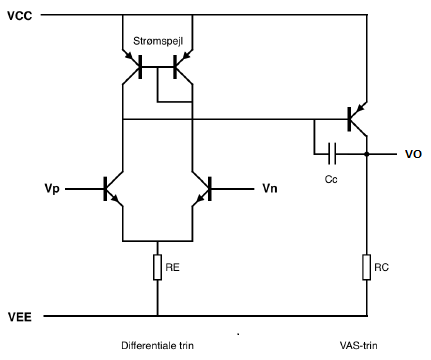
\includegraphics[width=0.9\linewidth]{graphics/vas}
	\caption{Trans-resistans forstærker (VAS).}
	\label{fig:VAS_forstærker}
\end{figure}
DC forstærkningen er således givet ved:
\begin{equation} 
A_{DC} = g_m \beta R_C
\end{equation}

Kondensatoren $C_C$ skaber en dominerende pol ved $f_0$, som sikrer stabilitet.

\begin{equation} 
f_0 = \dfrac{1}{2 \pi \beta R_C C_C}
\end{equation}

Slew-raten (SR) begrænses af kondensatoren og strømmen $I_E$.

\begin{equation} 
SR = \dfrac{I_E}{C_C}
\end{equation}

\begin{figure} [H]
	\centering
	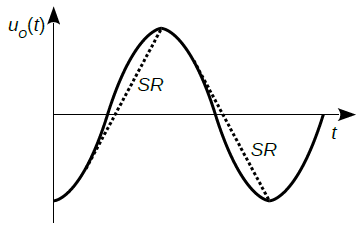
\includegraphics[width=0.65\linewidth]{graphics/slewrate}
	\caption{Operationsforstærkerens slew rate.}
	\label{fig:slewrate}
\end{figure}

Den dominerende pol giver stabilitet, men begrænser også hvor hurtigt udgangen kan flyttes. Hvis værdien forsøges overskredet bliver signalet forvrænget.

\textbf{Lave frekvenser}
\begin{equation} 
U_O = g_m \beta R_C(U_P-U_N)
\end{equation}

\textbf{Høje frekvenser}
\begin{equation} 
U_O = \frac{g_m}{j \omega C_C}(U_P-U_N)
\end{equation}

\subsection{AC forhold og stabilitet}
\begin{itemize}
	\item En operationsforstærker har mindst to poler.
	\item En tilbagekoblet operationsforstærker skal have en dominerende pol for stabilitet.
	\item Ved tilbagekobling giver det en overføringsfunktion af mindst andet orden og det kan give problemer med stabilitet.
	\item For at gardere sig kan man vælge den dominerende pol $f_0$ så lavt at systemet bliver ubetinget stabilt.
	\item Miller transformation udføres for at finde modstande og kapaciteter, der resulterer i poler.
\end{itemize}

Polen mellem differentialtrinnets T1 til T4 og VAS-trinnets T5 bliver normalt ofret ved at inkludere $C_C$ der sænker polens frekvens så den udgør operationsforstærkerens dominerende pol. Polens frekvens er som regel lavere end 1 kHz. 

Der er en fordel ved valget idet kapaciteten $C_{\si{\micro}}$ fra kollektor til basis ved T5 bliver stort set uden betydning. 
Det er væsentligt fordi operationsforstærkerens egenskaber ved høje frekvenser defineres af netop denne kapacitet.
Det betyder at kondensatoren er aktiv i hele frekvensområdet den dominerende pol. 
Transistorens kapacitet $C_{\si{\micro}}$ er spændingsafhængig og vil derfor introducere harmonisk forvrængning, men ved at parallelkoble $C_{\si{\micro}}$ med en stabil kapacitet $C_C$ kan forvrængningen sænkes. 


Den hastighed udgangen kan flyttes med, altså slew raten, begrænses af strømmen $I_E$ og kapaciteten $C_C$ som beskrevet tidligere. 
Et design af en operationsforstærker bliver derfor et kompromis mellem at opnå en hurtig forstærker, altså en stor slew rate, og stabilitet, altså en lav værdi af GBP. 

\paragraph{Udgangstrinnet} fra operationsforstærkeren benytter oftest to eller flere transistorer koblet som emitterfølger. Trinnets opgave er at kunne levere (eller optage) en stor strøm til (fra) belastningen $R_L$ samt at isolere det relativt høje impedansniveau ved kollektor af T5 fra belastningens varierende værdi. Modstanden $R_C$ er faktor i udtrykket for åben-sløjfe forstærkningen $A_{OL}$ og ønskes derfor til en høj værdi. Det giver så til gengæld en pol ved udgangen af forstærkertrinnet.

\subsection{Offset-fejl og støj}

\newpage
\section{Dioden}
Dioder og transistorers egenskab er PN overgangen der kun tillader en elektrisk strøm at løbe i én retning.

\begin{itemize}
	\item En populær model er at spændingsfaldet har en konstant værdi på 0,7 V.
	\item Dioden er afbrudt når anodens spænding er lavere end katodens spænding.
	\item Dioden repræsenteres af en spændingsforskel på 0,7 V når anodens spænding er højere end katoden og der løber en strøm.
	\item Spændingsfaldet over dioden i lederetningen udnyttes i kredsløb som en reference for det øvrige kredsløb. Det kaldes for et kunstigt nulpunkt.
	Andre kredsløb måler spændingsfaldet som et udtryk for temperaturen da der er en relation på cirka \SI{2}{\milli\volt\per\degreeCelsius} for dioder uanset konstruktionen.
\end{itemize}


\subsection{PN overgangen}
\begin{itemize}
	\item Diodens N halvleder har et overskud af frie elektroner.
	\item Diodens P halvleder har et overskud af flytbare huller. 
	\item Diffusionen af elektroner danner et elektrisk felt som modvirker diffusionen. 
	\item En ekstern spændingskilde kan ændre på det elektriske felt og derved styre strømmen i dioden.
\end{itemize}

En elektron kan slås fri fra den yderste skal hvis atomet får tilført tilstrækkelig energi som for silicium er 1,125 eV.
Energien kan komme fra en temperatur på cirka \SI{300}{\kelvin} (\SI{27}{\degreeCelsius}), fotoner fra lyskilder og elektromagnetiske felter eller kollision med andre partikler som radioaktivitet og avalance-diode.

\begin{figure} [H]
	\centering
	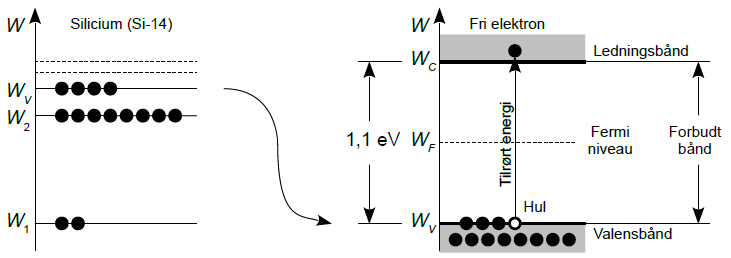
\includegraphics[width=\linewidth]{graphics/energimodel}
	\caption{Energimodel af grundstoffet silicium der har 14 elektroner fordelt i tre skaller.}
	\label{fig:energimodel}
\end{figure}

Afstanden mellem den øvre grænse af valensbåndet og den nedre grænse af ledningsbåndet betegnes ”det forbudte bånd”. Elektroner kan ikke opholde sig i dette energiområde.
Enten har elektronen fået energi nok til at foretage springet eller også har den ikke fået tilført energi nok.

\begin{figure} [H]
	\centering
	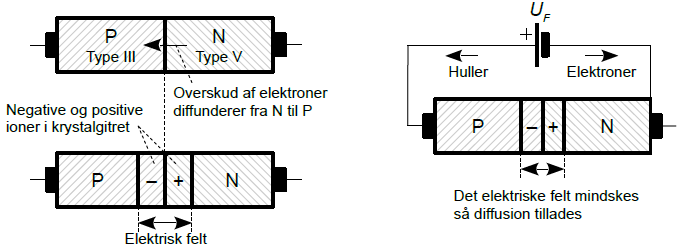
\includegraphics[width=\linewidth]{graphics/PN_overgang}
	\caption{PN overgangen.}
	\label{fig:pnovergang}
\end{figure}

Hvis der påtrykkes en ekstern spænding med plus ved P og minus ved N vil det tilføre frie elektroner til N halvlederen som rekombinerer med ionerne ved PN overgangen og mindsker det elektriske felt.
Derved kan elektroner diffundere gennem PN overgangen og rekombinere med hullerne i P. Det skaber et underskud af huller i P som gendannes ved at elektroner løber til batteriets positive pol. \textbf{Der løber en elektrisk strøm i dioden}. \\

Hvis det eksterne batteri vendes om vil det derimod trække
elektroner ud fra N hvorved det elektriske felt øges og blokerer for en strøm. \textbf{Dioden spærrer.}

\subsection{Diodens I-U karakteristik}
Diodens karakteristik I(U) har tre vigtige områder. 
\begin{itemize}
	\item I det ledende område er strømmen en eksponentiel funktion af diodens spænding.
	\item I det spærrende område er strømmen meget lille, men varierer nu eksponentielt med temperaturen. 
	\item I zener området vil diodens strøm vokse voldsomt når spændingen over dioden overskrider en grænse givet af fremstillingsprocessen.
	\item Relationen er eksponentiel og strømmen vokser en dekade
	ved en ændring af spændingen over dioden på cirka 60 mV for n = 1. Relationen vil almindeligvis holde over et område på seks dekader fra 10 nA til 10 mA for småsignaldioder.
\end{itemize}

\begin{figure} [H]
	\centering
	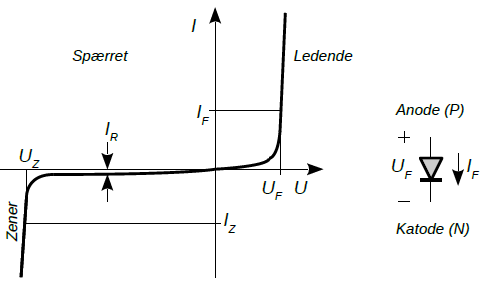
\includegraphics[width=0.9\linewidth]{graphics/I-U_karakteristik}
	\caption{Diodens karakteristik I(U).}
	\label{fig:I-U_karakteristik}
\end{figure}

\subsection{Modeller - AC/DC}
\paragraph{DC modellen} for dioden har en DC modstandsværdi, $R_D$, som resulterer i et større målt spændingsfald, $U_D$, i lederetningen ved en given strøm $I_F$.

\begin{equation}
U_D = U_F + R_D I_F
\end{equation}

\begin{figure} [H]
	\centering
	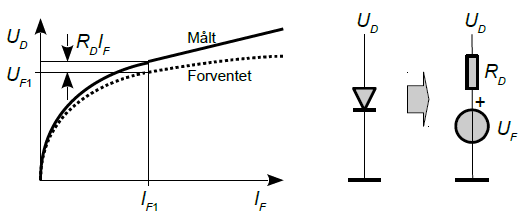
\includegraphics[width=\linewidth]{graphics/DC_diode}
	\caption{Diodens seriemodstand ved DC.}
	\label{fig:DC_diode}
\end{figure}

\newpage
\paragraph{AC modellen} for dioden hvor seriemodstanden er ubetydelig, kan dioden ses som en strømstyret modstand. 
Modstanden falder ved højere strømme.

\begin{equation}
r_D = \dfrac{U_T}{I_F}
\end{equation}

\begin{figure} [H]
	\centering
	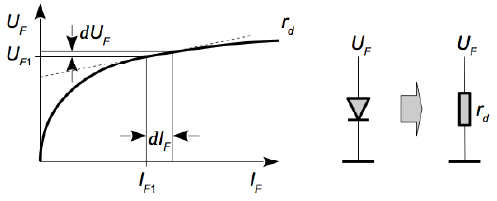
\includegraphics[width=\linewidth]{graphics/ACdiode}
	\caption{Diodens seriemodstand ved AC.}
	\label{fig:AC_diode}
\end{figure}

\subsection{Anvendelser}
\begin{itemize}
	\item Spændingskilde
	\item Motor - aflede strøm
	\item Kortslutningssikringer
	\item Ensretter 
\end{itemize}

\newpage
\section{Transistoren: DC}

\subsection{DC model}

\begin{figure} [H]
	\centering
	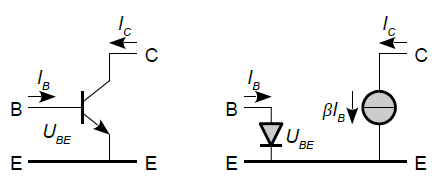
\includegraphics[width=0.8\linewidth]{graphics/transistor_DCmodel}
	\caption{Transistorens strøm er styret af base-emitter spændingen eller basisstrømmen.}
	\label{fig:transistor_DCmodel}
\end{figure}

\textbf{DC model 1 – Spændingsstyret}
\begin{itemize}
	\item Spændingen over transistorens base-emitter junction, $U_{BE}$, styrer kollektorstrømmen $I_C$.
	\item Basisstrømmen er ${\beta}$ gange mindre end kollektorstrømmen.
\end{itemize}

\begin{equation}
I_C = I_S \exp \dfrac{U_{BE}}{n U_T}
\end{equation}

\begin{equation}
I_B = \dfrac{I_C}{\beta}
\end{equation}

\textbf{DC model 2 – Strømstyret}
\begin{itemize}
	\item Basisstrømmen $I_B$ styrer kollektorstrømmen $I_C$.
	\item Strømforstærkningen ${\beta}$ er typisk mellem 100 og 1000 for småsignal transistorer.
	\item Effektransistorer forstærker 10 til 100 gange.
\end{itemize}
 
\begin{equation}
I_C = I_B {\beta}
\end{equation}

\begin{equation}
U_{BE} = n U_T \ln \dfrac{I_C}{I_S}
\end{equation}

\subsection{Forskellige typer (BJT, FET)}

\paragraph{BJT} er en bipolar transistor som fremstilles ud fra en diode ved at tilføje endnu et lag. 
Med et ekstra N lag på mod diodens anode kan elektronerne løbe videre i ledningsbåndet til nye N lag der kaldes for kollektor.\\
 
Hvis bredden af P laget er væsentlig mindre end rekombinationslængden vil hovedparten af elektronerne fortsætte fra emitter til kollektor.
De elektroner der rekomninerer i basis laget udgør transistorens basisstrøm. 

\begin{figure} [H]
	\centering
	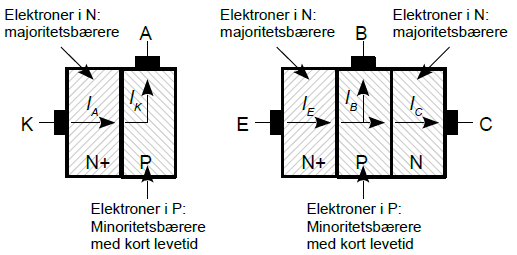
\includegraphics[width=0.95\linewidth]{graphics/bjt}
	\caption{En NPN transistors opbygning med emitter (N+), basis (P) og kollektor (N).}
	\label{fig:bjt}
\end{figure}

\begin{itemize}
	\item Der er to måder PN overgangene kan arrangeres på: NPN og PNP.
	\item De er komplementære transistorer.
	\item Meget ens, men lidt større diode spændingsfald ved en PNP.
\end{itemize}

\begin{figure} [H]
	\centering
	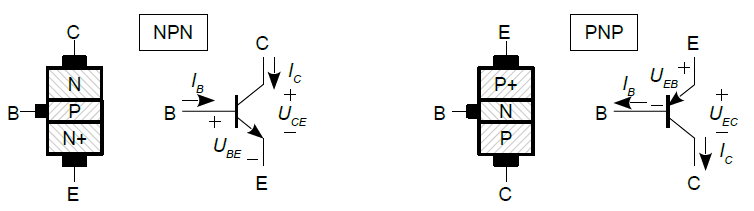
\includegraphics[width=\linewidth]{graphics/transistor}
	\caption{NPN og PNP transistor.}
	\label{fig:transistor}
\end{figure}
\newpage
\paragraph{JFET} er en betegnelse for junction field effect transistor. 
Den har tre elektroder der benævnes \textit{gate} for styreelektroden, \textit{source} for strømkilden og \textit{drain} for opsamling af
elektronerne. 

Styreelektroden gate er forbundet til kanalen mellem drain og source via en spærrende diode. 
Med en negativ spænding på gate i forhold til source vil det elektriske felt frastøde elektroner i nærheden af dioden. 

Modstanden af kanalen er givet ved antallet af frie elektroner.
Hvis kanalen indsnævres ved det elektriske felt fra gate vil der være færre elektroner og derved en højere modstandsværdi mellem source og drain.

\begin{itemize}
	\item Transistoren er åben uden spænding på gate.
	\item En negativ gate-source spænding vil begynde at begrænse drain-strømmen $I_D$.
	\item Transistoren er helt spærende ved den negative pinch off spænding: $U_P$.
\end{itemize}

\begin{figure} [H]
	\centering
	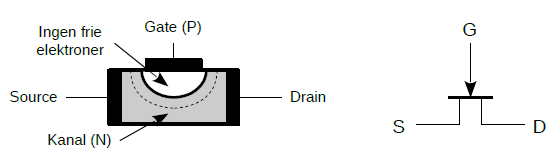
\includegraphics[width=\linewidth]{graphics/jfet}
	\caption{JFET transistor.}
	\label{fig:jfet}
\end{figure}

Kanalen mellem source og drain er i mange tilfælde symmetrisk og de to elektroder kan da ombyttes. Hvis det ikke er tilfældet tegnes pilen nærmest ved source.


\paragraph{MOSFET} er betegnelsen for en metal-oxide silicon field-effect transistor.

\begin{itemize}
	\item Mosfetten spærer for strøm når gate-spændingen $U_G < U_{TH}$.
	\item Der kan løbe strøm i drain når gaten lades op (det tager tid, som en kondensator).
	\item Gate kapaciteten begrænser hvor hurtigt den kan tænde/slukke.
\end{itemize}

\begin{figure} [H]
	\centering
	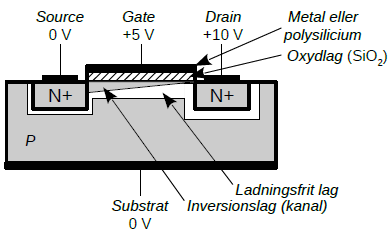
\includegraphics[width=0.7\linewidth]{graphics/mosfet}
	\caption{MOSFET transistor opbygning.}
	\label{fig:mosfet}
\end{figure}

\begin{figure} [H]
	\centering
	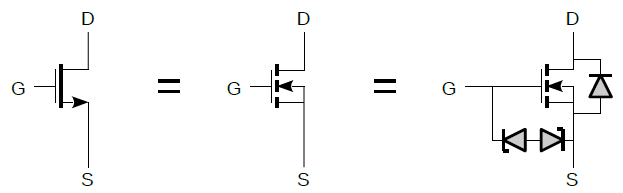
\includegraphics[width=\linewidth]{graphics/mosfet_symbol}
	\caption{MOSFET transistor symbol.}
	\label{fig:mosfet_symbol}
\end{figure}

\subsection{Anvendelser}
\textbf{Diodekobling}
\begin{itemize}
	\item Ved at korslutte basis og kollektor bliver transistoren en diode.
	\item Hyppigt brugt i IC design.
	\item Anvendes i strømspejlet.
\end{itemize}

\begin{figure} [H]
	\centering
	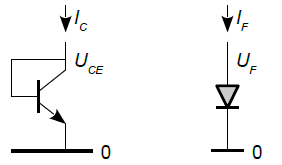
\includegraphics[width=0.6\linewidth]{graphics/diodekobling}
	\caption{Transistoren kan benyttes som diode.}
	\label{fig:diodekobling}
\end{figure}

\textbf{Strømspejl}
\begin{itemize}
	\item Strømmen I1 vil føre til en tilsvarende strøm I2.
	\item Der løber en lille basis-strøm, som i praksis vil føre til en fejl i I2.
\end{itemize}

\begin{figure} [H]
	\centering
	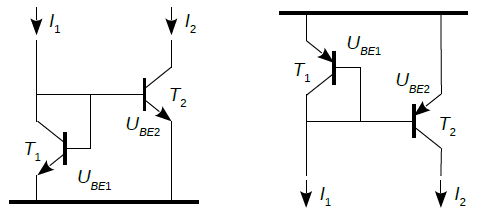
\includegraphics[width=0.8\linewidth]{graphics/currentmirror}
	\caption{Strømspejl placeret ved low side (venstre) og high side (højre).}
	\label{fig:currentmirror}
\end{figure}


\newpage
\section{Transistoren: AC}
\subsection{AC model}

DC-arbejdspunktet angives med $I_B$, $I_C$ og $U_BE$.\\

AC-værdierne angives med $i_B$, $i_C$ og $u_BE$.

\paragraph{Linearitet} kan for en transistor opnås ved at holde signalniveauet lavt. Arbejdspunktet må ikke kommer tæt på $I_C = 0 mA$ og må kun svinge få mV omkring dette arbejdspunkt. 
\begin{equation} 
I_C = g_m u_{BE}
\end{equation}

\begin{equation} 
i_C = I_S \exp \dfrac{u_{BE}}{n U_T}
\end{equation}

Strømmen i kollektor $i_C$ variererer proportionalt med $u_{BE}$ ved svagt signal.

\begin{equation} 
i_C = \dfrac{I_C}{n U_T} u_{BE}
\end{equation}

\begin{figure} [H]
	\centering
	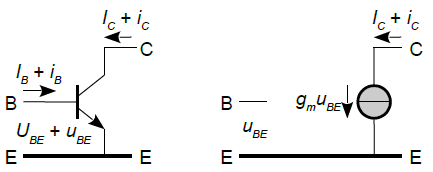
\includegraphics[width=0.75\linewidth]{graphics/ACmodel}
	\caption{Simpel AC model.}
	\label{fig:ACmodel}
\end{figure}

DC arbejdspunktet $I_C$ giver fundamentet for AC modellens vigtigste parameter: transkonduktansen.

\paragraph{Transkonduktansen} er proportionaliteten mellem småsignals-kollektorstrømmen $i_C$ som funktion af spændingen $u_BE$. 
Den beskriver ledningsevnen i siemens (S).\\

For at finde et arbejdspunkt hvor det er muligt at lave denne småsignals overførelse, laves en DC analyse hvor $I_C$  og $U_{BE}$ bestemmes. Ud fra disse kan transkonduktansen findes som:

\begin{equation} 
g_m = \dfrac{I_C}{U_T}
\end{equation}

\paragraph{Miller transformationen} 
Transistoren har en intern kapacitet $C_{\si{\micro}}$ i den spærrende diode i kollektor-basis og den begrænser den opnåelige båndbredde.
Ved et eksempel med en mikrofon forstærker vises Miller transformationen. Først oversættes kredsløbet til en AC model:
\begin{figure} [H]
	\centering
	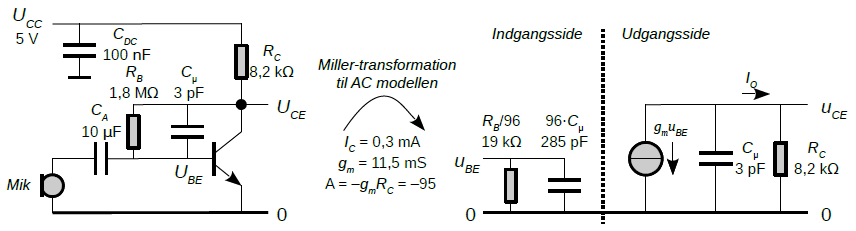
\includegraphics[width=\linewidth]{graphics/millertransformation}
	\caption{Mikrofonforstærker med kapaciteten $C_{\si{\micro}}$ indtegnet.}
	\label{fig:millertransformation}
\end{figure}
Fra AC modellen ovenfor ses det at forstærkningen må være 

\begin{equation} 
A = \dfrac{u_{CE}}{u_{BE}}
\end{equation}

$u_{CE}$ må for dette kredsløb være spændingsfaldet over $R_C$ da strømmen løber væk fra $I_o$.

\begin{equation} 
u_{CE} = -g_m u_{BE}R_C
\end{equation}

Dette indsættes i udtrykket for forstærkningen

\begin{equation} 
A = \dfrac{-g_m u_{BE}R_C}{u_{BE}}
\end{equation}

På billedet nedenfor er en mikrofon forstærker Miller transformeret

Først findes transkonduktansen for kredsløbet $I_C$ vælges til \SI{2}{\milli\ampere} i DC analysen:

\begin{equation} 
g_m = \dfrac{I_C}{u_T} = \dfrac{\SI{2}{\milli\ampere}}{\SI{26}{\milli\volt}} = \SI{0.08}{\siemens}
\end{equation}

Dernæst findes forstærkningen i kredsløbet:

\begin{equation} 
A = -g_m R_C = g_m \SI{1.25}{\kilo\ohm} = -95
\end{equation}

Herefter findes indgangs impedansen af kredsløbet:
Hvis modstanden $R_B$ skal have samme strøm gennem sig når den er sat til 0V må den ændres i værdi, da der over den er et spændingsfald på
$u_{CE}-u_{BE}$ hvilket ikke er lig $u_{BE}-0V$. Det nye spændingsfald er 1-A gange mindre og får at få den samme strøm må $R_B$ ændres til

\begin{equation} 
R_B = \dfrac{R_{BM}}{1-A}
\end{equation}

\begin{equation} 
R_I = R_{BM} = \dfrac{\SI{270}{\kilo\ohm}}{1-(-95)} = \SI{2.8}{\kilo\ohm}
\end{equation}

Næst findes udgangsimpedansen:
Da $R_B$ set fra indgangens synspunkt har en meget lav spænding (A gange mindre ind på udgangen) på indgangen, kan dette ses som 0V og i dette tilfælde er $u_{CE}-u_{BE} = u_{CE}-0V$, derfor skal modstanden ikke ændres ved Miller transformationen, heller ikke $R_C$. 

\subsection{Koblingstyper og deres egenskaber}
(forstærkning, ind- og udgangsimpedans)

\subsection{Støj og forvrængning}
\begin{itemize}
	\item Forstærkeren er ikke støjfri.
	\item Termisk støj fra modstandene $e_{nR}$.
	\begin{itemize}
		\item Signalkildens modstand $R_G$.
		\item Basismodstanden $r_x$.
	\end{itemize}
	\item Haglstøj fra strømmene i basis og kollektor.
	\begin{itemize}
		\item Basis $i_{nB}$
		\item Kollektor $i_{nC}$
	\end{itemize}
\end{itemize}

Transistorens forvrængning kan holdes til \SI{1}{\percent} THD (total harmonic distortion) ved at indgangssignalet varierer med mindre end 1mA. Dette skyldes transistorens eksponentielle karakteristik.


\end{document}